%%%% ijcai17.tex

\typeout{Motif-Aware Graph Embeddings}

% These are the instructions for authors for IJCAI-17.
% They are the same as the ones for IJCAI-11 with superficical wording
%   changes only.


\documentclass{article}
% The file ijcai17.sty is the style file for IJCAI-17 (same as ijcai07.sty).
\usepackage{ijcai17}
\usepackage{amsthm}
\usepackage{amssymb}
\usepackage{amsmath}
% Use the postscript times font!
\usepackage{times}
\usepackage{graphicx} 
\usepackage[ruled,vlined]{algorithm2e}
\usepackage{multicol}
\usepackage{float}
\usepackage{dsfont}

% the following package is optional:
%\usepackage{latexsym}

\DeclareMathOperator*{\argmin}{arg\,min}
\DeclareMathOperator*{\argmax}{arg\,max}


\theoremstyle{definition}
\newtheorem{definition}{Definition}[section]

\title{Motif-Aware Graph Embeddings}

\author{Anonymous authors}

\begin{document}

\maketitle

\begin{abstract}

  In this paper, we propose our motif-aware approaches to the 
  unsupervised network embedding and semi-supervised network labeling 
  task. Our first algorithm is an unsupervised network embedding 
  algorithm which uses the most statistically significant network motif 
  as the guiding pattern for random walks to generate network context. We 
  then use a Skipgram neural network to learn the latent network node 
  representations from the generated context via Noise Contrastive 
  Estimation. The second algorithm employs the Graph Convolution Network 
  model on motif Laplacian matrices to inject the higher-order network 
  structure into the neural network. Both of our algorithms utilize the 
  higher-order organization (i.e. motifs organization) of complex 
  networks. We demonstrate the effectiveness of our algorithms in 
  comparison to other state-of-the-art network embedding algorithms.

\end{abstract}

\section{Introduction}

\subsection{Complex network and machine learning}

Network modelings have been an essential tool for a wide
range of scientific fields
\cite{physicnet,molecule,motifblockmilo,juremotif}. 
Based on the system's network structure, 
scientists can make predictions and explanation
about the system's behavior. For example, in biology, the
study of neuronal systems connectivity indicated
that the component arrangement of a neural system is optimized
for short processing paths rather than wiring lengths
\cite{kaiser2006nonoptimal}. Similarly, social network
analysis provides communities structures well as 
social interaction patterns 
\cite{west2014exploiting,barabasi2014network}. 
However, along with the information explosion, analyzing
large network-structured datasets poses a great challenge 
for traditional network analysis methods in term of 
scalability and complexity. To deal with such challenge,
one promising approach is to apply machine learning methods 
(especially deep learning) to network problems.

Bridging the gap between network-structured data and typical
data structure for machine learning is also a challenge. 
Due to the irregularity in the network-structured data, 
it is desirable to have a \emph{meaningful}
network representation for machine learning applications. 
Learning network representation in real vector spaces can be
viewed as manifold learning (non-linear dimensionality reduction),
and commonly known as \emph{network embedding} in the literature.
In this report, we propose the use of network motifs into learning
a high-quality network embedding. The \emph{embedding quality} in this
context is justified by how well a common machine learning model performs 
on the learned embeddings.

\begin{figure} \label{fig:cartoon}
    \centering
    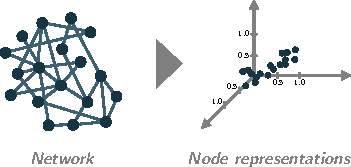
\includegraphics[width=0.8\linewidth]{cartoon_emb}
    \caption{Learning a latent representation of nodes from the network structure. In this figure, the example network is embedded to a 3-dimensional real vector space.}
\end{figure}

\subsection{Motifs in complex network}

There are three scales of network analysis: macroscopic, mesoscopic, 
and microscopic. In the macroscopic scale, we consider a network as a 
whole to study its macro-properties such as robustness 
\cite{callaway2000network}, or dynamics \cite{barabasi2014network}.
In contrast, the microscopic scale studies the pair-wise interactions
between nodes in a network which is specific to a given system 
\cite{physicnet}. In between macroscopic and microscopic, the mesoscopic 
scale considers the network is a composition of subgraphs. 
In many fields of research, especially computational biology, the
mesoscopic components are called \emph{motifs}, and it is common
to think of them as building blocks of a complex system 
\cite{motifblockmilo}.

\begin{definition}{\emph{Network motif}}:
Given a graph $G = (V,E)$, define a subgraph $G' = {V', E'}$ with $V' 
\subseteq V$;
$E' \subset E$ s.t. $i,j \in V' \forall e_{ij} \in E'$ and $|V'| \ll |V|$. 
Recurring subgraphs are called \emph{network motif} when they are 
statistically significant.
\end{definition}

\begin{figure} 
    \centering
    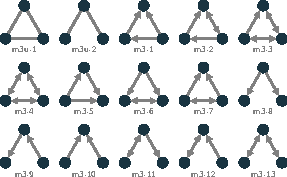
\includegraphics[width=0.9\linewidth]{m3}
    \caption{Size-3 motifs}
    \label{fig:m3}
\end{figure}

Also referred as the higher-order organization by \citeauthor{juremotif}, 
network motifs are believed to represent the underlying mechanism of a 
complex system 
\cite{netmotif,alon2006introduction,mangan2003structure}. 
For instance, the directional bi-fan motif (figure \ref{fig:m4}: m4-1)
and its simplified unidirectional version (m4u-3) are crucial in a citation 
network. This bi-fan motif is also intuitively sensible in citation network 
as it represents the citation mechanism. 
The correlation of recurring subgraphs and system 
functionality has been studied extensively in biological systems such as 
transcription networks \cite{mangan2003structure} and brain 
networks \cite{brainnetheuvel,honey2007network}. As networks motifs
have been recognized as the fundamental building block of a complex
systems, using them as a structural guidance for machine learning
on network data can yield positive improvements.

Our main idea in this paper is to construct the motif co-occurrence matrix
from a given network, and use it as: 1. An adjacency matrix describing a 
motif network for random walks; 2. A mean to compute motif Laplacian and 
Fourier basis for the graph convolution operation. Section 2 describes the 
related work on network motif conductance and network embedding. We give 
detail of our algorithms in section 3. The experimental setup and results 
are given in section 4 and 5 respectively. We discuss the relationship 
between our two proposed algorithms and their limitations in section 6.

\section{Related work}

In this section, we introduce the recent developments regarding unsupervised 
network embeddings, semi-supervised node labeling, and motif analysis.

\begin{figure} 
    \centering
    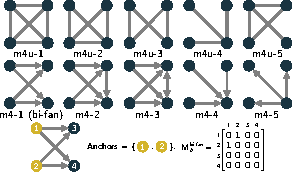
\includegraphics[width=0.9\linewidth]{m4}
    \caption{Size-4 motifs and anchor set example}
    \label{fig:m4}
\end{figure}

\subsection{Unsupervised Network Embedding}

Traditionally, network embedding can be obtained via graph 
factorization methods. However, matrix factorization methods such as
Spectral Clustering or Non-negative Matrix Factorization are 
shown to be unscalable due to the complexity of the algorithms 
\cite{deepwalk,eigmaps,pca}. Recently, several feasible network
embedding algorithms have been proposed such as \emph{Deepwalk}
\cite{deepwalk} or \emph{Node2Vec} \cite{node2vec}. These network embeddings 
algorithms learn high-quality node representation while having low time
complexity compared to traditional methods. In the context of graph embedding, we 
justify the \emph{embedding quality} by how well a common machine learning model 
performs on the learned embeddings. 

Based on the Skipgram model \cite{skipgram} in natural language 
processing, \citeauthor{deepwalk} proposed their scalable graph embedding 
algorithm named \emph{Deepwalk}. Their results on node classification proved the 
effectiveness of \emph{Deepwalk} in learning a lower dimensionality 
representation of a complex network. Subsequent work to DeepWalk further 
improved node classification accuracy by modifying graph context 
generation process \cite{line,grarep,planetoid,node2vec}. Generally, these
algorithms optimize the following objective:
\begin{equation} 
\mathcal{O} = \argmax_{W^{\scalebox{0.75}{emb}}}\ ( 
\ell_{\scalebox{0.75}{random walk}}),
\label{eq:deepwalkobj}
\end{equation}
where $\ell_{\scalebox{0.75}{random walk}}$ represents the log-likelihood
of the network context generated by random walks on the given network. We have
the pairwise potential between a \emph{context} vertex $v_c$ and a \emph{target}
vertex $v_t$ as follow:
\begin{equation}
\begin{aligned}
	\phi_{v_t,v_c} &= \exp{( \langle \omega_{v_c} ,  \omega_{v_t} \rangle )} \\
	\ell_{\scalebox{0.75}{random walk}} &= \sum_{v_t,v_c}
	\log{(\frac{\phi_{v_t,v_c}}{\sum_{k \in V} \phi_{v_k,v_t}})}
\end{aligned}
\label{eq:deepwalkprob}
\end{equation}
In here, $\langle \cdot , \cdot \rangle$ denotes the inner product; $\omega_v$ 
denotes the real vector representation of node $v$; and $W^{\scalebox{0.75}{emb}}$
is the output matrix containing all real vector representations. Although the 
log-likehood given by equation \ref{eq:deepwalkobj} is tractable, computing the
normalization factor still remains an intractable task. Therefore, several 
approximation methods such as hierarchical softmax \cite{hs,deepwalk} or noise
contrastive estimation \cite{nce,node2vec} were used to further boost the
computational speed of the algorithms of this category. The obtained embedding
matrix will be used as a feature matrix for various machine learning algorithms
such as node classification (Multi-class Linear Regression model) or link 
prediction.

\subsection{Semi-supervised Network Labeling}

\emph{Planetoid}, proposed by \citeauthor{planetoid}, works slightly different to 
other Skipgram-based models. Instead of generating graph context only from the
network structure, \emph{Planetoid} also samples nodes based on training labels. 
Furthermore, \emph{Planetoid} injects the network node's feature vectors for better 
embedding and node labeling results. \emph{Planetoid} can be considered an
improvement of \emph{SemiEmb}, proposed in \cite{weston2012deep}. Another semi-
supervised learning model similar to \emph{Planetoid} is Graph Convolutional 
Networks (GCN) \cite{gcn}. GCN uses the graph convolutional operation as a 
transformation for feature vectors on a network. By stacking these convolutional 
operation into a neural network, the authors of GCN has been able to achieve 
remarkable accuracy in node classification and link prediction results 
compared to the previous unsupervised and semi-supervised algorithms. Moreover, the
running time for GCN was superior compared to other algorithms such as 
\emph{Deepwalk} or \emph{Planetoid}. In the following paragraphs, we present 
the details for \emph{GCN}.

The convolution on a graph $G$ of a function of the graph 
Laplacian $g_{\theta}$ (also called a filter or a kernel) 
and a signal $x$ is defined as:
$$g_{\theta} \ast x = g_{\theta}(\mathcal{L}) x,$$
where the normalized Laplacian $\mathcal{L} = U \Lambda U^\top$; 
$U$ is the Fourier basis and $\Lambda$ is called the frequencies of the graph. 
Graph convolution has been shown effective in processing
graph-structured data, and also argued to be the generalization
of convolutional networks
\cite{shuman2013emerging,defferrard2016convolutional,gcn}.
In practice, given a graph where each node has a feature vector,
we can treat the feature vector of the graph as signals. The output $y$
of these "signals" filtered by $g_\theta$ on the graph is given by
the graph convolution and its inverse: 
\begin{equation}
\label{eq:graphconv}
y = g_\theta (U \Lambda U^\top) x = U (g_\theta(\Lambda) U^\top)x
\end{equation}
Computing equation \ref{eq:graphconv} is computationally expensive
due to the matrix multiplication and eigenvector decomposition operations.
Therefore, fast estimation methods such as Chebyshev polynomial was suggested
in \cite{hammond2011wavelets}. Under the assumption
$\lambda_{\scalebox{0.75}{max}} \approx 2$, \citeauthor{gcn} further
proposed the linear approximation for filtering signals $X$ on a graph:
\begin{equation}
\label{eq:gcnapprox}
y \approx \theta \left( I + D^{-1/2}
A D^{-1/2} \right)
\end{equation}
Following the graph convolution approximation above, the \emph{GCN} neural network
model can be described by the forward computation and the loss function:
\begin{equation}
\label{eq:gcnnn}
\begin{aligned}
	Z_{\scalebox{0.75}{forward}} &=
\mbox{softmax}\left(\hat{A} \mbox{ ReLU}(\hat{A}XW^{(0)})W^{(1)}\right) \\
	loss &= -\sum_{l \in \mathcal{Y}_L} \sum^F_{f=1} Y_{lf}\mbox{ln} Z_{lf} \\
\end{aligned}
\end{equation}
where $W$ is the weight matrix for hidden layer (0) and output layer (1);
$\hat{A} = \tilde{D}^{-1/2} \tilde{A} \tilde{D}^{-1/2}$ is called the
\emph{Renormalization Trick} by the authors \cite{gcn}. The loss function here
is the cross-entropy error over all labeled samples similar to the model proposed
in \cite{planetoid}. The neural network is trained using Adam \cite{adam} with
back-propagation. 

\begin{figure*}
    \centering
    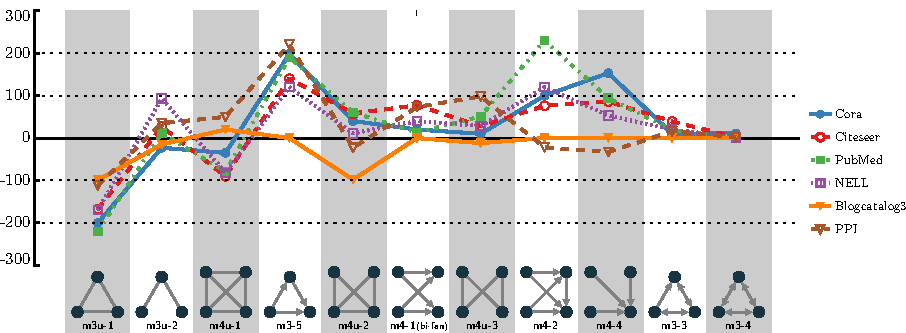
\includegraphics[width=0.9\linewidth]{sigm}
    \caption{Significant graph for selected motifs (size-3 and size-4)}
    \label{fig:sigm}
\end{figure*}

\subsection{Motif Conductance}

\begin{algorithm}[h] \label{al:madj}
\KwData{Graph $G = (V,E)$}
\KwIn{isBinary, $\mathbf{m}$, $\mathcal{A}$}
\KwOut{$M^{\mathbf{m}}$}
\Begin{
    diam $\leftarrow$ Diameter($\mathbf{m}$, $\mathcal{A}$); \\
    $V$ $\leftarrow$ $G$.nodes(); \\
    \For{$i$ $\in$ nodes} {
        $G'$ $\leftarrow$ induced graph from BFS(node, diam); \\
        \For{$j$ $\in$ $G'$.nodes()} {
            \uIf{(i,j) satisfies $\mathcal{A}$} {
                $c \leftarrow \mbox{count } \mathbf{m} \mbox{ in } G'$; \\
                \uIf{isBinary} {
                	$M_{i,j}^{\mathbf{m}} \leftarrow 1$ if $c > 0$ else $0$;\\
                } \uElse {
                	$M_{i,j}^{\mathbf{m}} \leftarrow c$;\\
                }
            } \uElse {
                $M_{i,j}^{\mathbf{m}} \leftarrow 0$; \\
            }
        }
    }
\KwRet{$M^{\mathbf{m}}$}
}
\caption{Motif co-occurrence matrix generation}
\end{algorithm}

As an generalization of \emph{network conductance} (also graph conductance 
or Cheeger constant of a graph), \citeauthor{juremotif} proposed
the concept of \emph{motif conductance} in \cite{juremotif}. Similar to
network conductance, motif conductance is a \emph{score} for a cut 
$(S, \bar{S})$ targeting a motif $\mathbf{m}$:
\begin{equation*}
	\phi_{\mathbf{m}}(S) = \frac{\mbox{cut}_{\mathbf{m}}(S,\bar{S})}{\min[\mbox{vol}_{\mathbf{m}}(S), \mbox{vol}_{\mathbf{m}}(\bar{S})]},
\end{equation*}
where $S$ is a node set in a network $G$; $\bar{S}$ is the complement
of $S$; $\mbox{vol}_{\mathbf{m}(S)}$ is the number of motif instance
endpoints in $S$. Intuitively, minimizing the motif conductance is
equivalent to minimizing the number of motifs $\mathbf{m}$ gets 
\emph{split} by the cut. A motif is split when there is at least one
anchor node in $S$ and at least one in $\bar{S}$. \citeauthor{juremotif}
then perform motif analysis and graph clustering based on this
definition of motif conductance. Their result further confirms the
structural role of motifs in a complex network. It also hinted that there
is a strong motif structure within a community, which we can use as
prior knowledge for solving problems on networks.

\begin{definition} \emph{Motif co-occurrence matrix}:
Given a graph $G = (V,E)$, in which $v \in V$. The motif co-occurrence 
matrix of a motif $\mathbf{m}$ is given by:
$$M_{i,j}^{\mathbf{m}} = \sum_{(v, \chi_{\mathcal{A}}(v)) \in \mathbf{m}} \mathbf{1}({i,j} \subset \chi_\mathcal{A}(v))$$
In here, $\mathcal{A}$ represents the anchor set; 
$(v, \chi_{\mathcal{A}}(v))$ represents pairs of node $v \in V_G$ and the 
other anchor nodes generated by $\chi_\mathcal{A}$. If the anchor node set 
$\mathcal{A}$ is empty, all motif co-occurrence is counted toward the 
motif co-occurrence matrix $M$. Otherwise, only nodes in the anchor set 
will be counted. Figure \ref{fig:m4} illustrates the bi-fan motif and 
its anchor set. Algorithm \ref{al:madj} provides detail for constructing
a motif co-occurrence matrix.
\end{definition}


\section{Methods}

In this section, we present the detail of our methods. Firstly,
we propose the basis for the network motif selection from a network.
Secondly, we present two approaches employing motif patterns to
learn graph embeddings: \emph{motifwalk} and \emph{m-gcn}.

\subsection{Motif Analysis and Motif Convolution}

In the previous section, we have explained the importance of
network motifs in network analysis. In this section, we present
the metric for measuring network motif significance and the definition
of motif Laplacian.

In order to measure the importance of a network motif, we compare
the given network against a null model. The null model of an empirical 
network is an ensemble of randomly generated networks having the same 
number of nodes and edges as the network. For small networks with less 
than 10,000 edges, we generated 100 random networks as the ensemble of the 
null model. On the other hand, we generated 10 random networks for the 
null model of larger networks. The $z\mbox{-score}$ is given by:
\begin{equation*}
z\mbox{-score} = \frac{N_\mathbf{m}(G)-N_\mathbf{m}(G_{\scalebox{0.75}{random}})}{\sigma_\mathbf{m}(G_{\scalebox{0.75}{random}})}
\end{equation*}
where $N_\mathbf{m}(G)$ is the count of motif $\mathbf{m}$ in the 
empirical network; $N_\mathbf{m}(G_{\scalebox{0.75}{random}})$ is the mean 
of the null model; and $\sigma_\mathbf{m}(G_{\scalebox{0.75}{random}})$ is
the variance. The $z\mbox{-score}$'s values can range from 
$-\infty$ to $+\infty$. In practice, the most simple motifs (figure 
\ref{fig:m3}-m2,3,4) often have the highest frequencies and negative $z
\mbox{-score}$. We ignored such motifs in our analysis. We select the motif 
which has the highest positive $z\mbox{-score}$ because these motifs
highlight the difference between the empirical network and random 
networks. 

Convolution operations on a network can be viewed as a method to
incorporate the nodes' information (e.g. feature vectors) 
and the network structure. The Fourier basis and network frequencies of
a motif co-occurrence matrix is obtained through the eigenvalue
decomposition of the motif Laplacian matrix $\mathcal{L}_{\mathbf{m}}$:
\begin{equation} \label{eq:eigm}
\mathcal{L}_{\mathbf{m}} = U_{\mathbf{m}} \Lambda_{\mathbf{m}} 
U^{\top}_{\mathbf{m}}
\end{equation}
In here, $\Lambda_{\mathbf{m}} = diag(\lambda_{\mathbf{m}})$ is called the 
frequencies of the motif network; $\mathcal{L}_{\mathbf{m}}$ is the 
normalized motif Laplacian given by:
\begin{equation} 
\begin{aligned}
\mathcal{L}_{\mathbf{m}} &= D_{\mathbf{m}}^{-1/2} L_{\mathbf{m}} 
D_{\mathbf{m}}^{-1/2} \\
&= I - D_{\mathbf{m}}^{-1/2} M^{\mathbf{m}} D_{\mathbf{m}}^{-1/2}
\end{aligned}
\label{eq:eigm}
\end{equation}
where $L_{\mathbf{m}} = D_{\mathbf{m}} - M^{\mathbf{m}}$; $M^{\mathbf{m}}$
is the motif co-occurrence matrix; and $D_{\mathbf{m}} = \mbox{diag} 
( \sum_j M^{\mathbf{m}}_{i,j} )$.

$U_{\mathbf{m}}$ from equation \ref{eq:eigm} is the Fourier basis of the 
network motif structure which is used for motif convolution. Given signal
$x \in \mathds{R}^n$ on a network, the motif Fourier transform is defined
as $\hat{x} = U_{\mathbf{m}}^{\top}x$, and its inverse as 
$x = U_{\mathbf{m}}\hat{x}$. It follows that the output of signal $x$
filtered by a function of graph Laplacian $g_{\theta}(L)$ parameterized
by a set of coefficient $\theta$ is given by:
\begin{equation}
\begin{aligned}
y &= g_{\theta} \ast x =  g_\theta (U_{\mathbf{m}} \Lambda_{\mathbf{m}} U_{\mathbf{m}}^\top) x \\
&= U_{\mathbf{m}} (g_\theta(\Lambda_{\mathbf{m}}) U^\top_{\mathbf{m}})x
\end{aligned}
\label{eq:filter}
\end{equation}   

Due to the complexity of eigenvector decomposition and matrix 
multiplication, we use the linear formulation suggested in \cite{gcn} to 
estimate the costly convolution operation: 
\begin{equation} \label{eq:linear}
\begin{aligned}
y &= g_{\theta'} \ast x \approx \sum_{k=0}^K \theta'_k T_k(\tilde{L})x \\
&\approx \theta_0' x + \theta_1 (L - I) = \theta_0' x - \theta_1' D^{-1/2}_{\mathbf{m}}
M^{\mathbf{m}}D^{-1/2}_{\mathbf{m}} \\
&\approx \theta \left( I + D^{-1/2}_{\mathbf{m}}
M^{\mathbf{m}}D^{-1/2}_{\mathbf{m}} \right)
\end{aligned}
\end{equation}

\subsection{Biased Random Walk}

Previous Skipgram-based graph embedding models employ random
walks for graph context generation. To improve the embedding results,
structure-aware context generation methods were proposed in 
\cite{line,node2vec}. However, the limitation of \emph{LINE} lies at the 
fact that it only consider the second-order proximity (bi-fan motif), and  
\emph{node2vec} requires the costly cross-validation grid search for its hyper-
parameters $p$ and $q$. To solve the above-mentioned problems, we propose 
a biased random walk algorithm for graph context generation which can be 
considered the generalization of \emph{LINE} and \emph{Deepwalk}. Since 
our algorithm decides the walking pattern supported by the most significant 
network motif before performing context generation, our method has the 
simplicity of \emph{Deepwalk} while having the structure-aware context as 
of \emph{LINE} and \emph{node2vec}.

Our \emph{motifwalk} algorithm has two steps: motif adjacency matrix
construction and context generation. Firstly, we construct a binary
motif co-occurrence matrix from the given network. We select the motif
pattern as described in the previous section. Since the constructed matrix 
accounts the co-occurrence of network node pairs in a motif, it is a 
symmetric matrix. Secondly, after having the motif adjacency matrix, 
we run random walks on this new network induced by the adjacency matrix
for motif context generation. The obtained motif context is used jointly 
with random walks context generated with the original network to train an 
embedding skipgram model. Algorithm \ref{al:madj} and algorithm 
\ref{al:cgen} describe the \emph{motifwalk} algorithm.
\begin{algorithm}[h] \label{al:cgen}
\KwData{Graph $G = (V,E)$, Motif Graph $G_{\mathbf{m}} = (V,E)$}
\KwIn{length, nwalk, nmwalk}
\KwOut{context}
\Begin{
    context $\leftarrow$ [~]; \\
    $V$ $\leftarrow$ G.nodes(); \\
    nodes $\leftarrow$ Shuffle($V$); \\
    \For{node $\in$ nodes} {
        walks $\leftarrow$ [~]; \\
        \For{i=0; i $<$ nwalk; ++i} {
            walks += RandomWalk(graph=$G$, \mbox{~~}start=node, len=length);
        }
        \For{i=0; i $<$ nwalk; ++i} {
            walks += RandomWalk(graph=$G_{\mathbf{m}}$, \mbox{~~}start=node, len=length);
        }
        context += walks;
    }
\KwRet{context}
}
\caption{Motif-aware graph context generation}
\end{algorithm}

Similar to other Skipgram-based models, \emph{motifwalk} is an unsupervised
algorithm which learns graph embedding through an optimization process. 
Since there is two network contexts generated in our algorithm, the 
objective function is given by:
\begin{equation} 
\begin{aligned}
&\mathcal{O} = \argmax_{W^{\scalebox{0.75}{emb}}}\ (\gamma 
\ell_{\scalebox{0.75}{random walk}} + (1-\gamma) \ell_{\scalebox{0.75}
{motif walk}}) \\
\end{aligned}
\label{eq:mloss}
\end{equation}
where $\ell_{\scalebox{0.75}{random walk}}$ and $\ell_{\scalebox{0.75}
{motif walk}}$
are the log-likelihoods of the network contexts generated by
random walk and motif walk respectively; $\gamma$ is a hyper-parameter
controlling the ratio between random walk. $\gamma$ is selected 
empirically based on the ratio between edges in the motif network and edges
in the given network. The likelihood
of a \emph{target} vertex $v_t$ in the context of vertex $v_c$ is given
in equation \ref{eq:deepwalkprob}. We use negative sampling with noise
contrastive estimation loss as suggested in \cite{skipgram} for normalization
factor estimation. The output of \emph{motifwalk} is a set of real 
vectors representing each node in the given network. These vectors encode 
the underlying structural relationship between network nodes and can be used as 
feature vectors for link prediction and node classification.

\subsection{Motif Convolutional Architecture}

In the previous section, we have defined the graph convolution
operation on motif co-occurrence matrix. We use the motif convolution
as the second layer in our motif convolutional network (m-gcn). Based on the 
linear approximation proposed by \citeauthor{gcn}, we define the forward
computation of our model as:
\begin{equation} \label{eq:mforward}
    \begin{aligned}
    Z_{\scalebox{0.75}{forward}} &= f(X,A,M) \\
    &= \mbox{softmax}(\hat{M} \mbox{ReLU}(\hat{A}XW^{(0)})W^{(1)}),
    \end{aligned}
\end{equation}
where $A$ and $M$ is a binary adjacency matrix and motif co-occurrence
matrix respectively; $\hat{A}$ and $\hat{M}$ are constructed by the
\emph{renormalization trick} as suggested in \cite{gcn}; $X$ contains
the feature vectors for each graph node; $W^{(0)}$ and $W^{(1)}$ are
learnable variables. We use Adam \cite{adam} with back-propagation 
to optimize the cross-entropy loss $E$:
\begin{equation}
	E = -\sum_{l \in \mathcal{Y}_L} \sum^F_{f=1} Y_{lf}\mbox{ln} Z_{lf}
	\label{eq:mloss}
\end{equation}
This formulation is the same as equation \ref{eq:gcnnn}. The weight $W$ is updated
by the following rule:
\begin{equation}
	\frac{\partial E}{\partial W^{(k)}_{i,j}} = \sum^S_{s=1} [x]^\top \frac{\partial E}{\partial y_{k,j}},
	\label{eq:mback}
\end{equation}
where $W^{(k)}$ is the weight matrix of layer $k$; $y_{k,j}$ is the 
$j^{\scalebox{0.75}{th}}$ output feature map of the sample $s$. 

\section{Experiments}

To compare \emph{motifwalk} performance with other unsupervised graph
embedding models, we have chosen the node labeling task on various
type of networks (with ground-truth node labels). In this paper, we
compare the performance of \emph{motifwalk} to \emph{Spectral Clustering}, 
\emph{Deepwalk} \cite{deepwalk}, \emph{node2vec} \cite{node2vec}. 
Table \ref{t:ungraph} gives the networks' statistics. The second model 
\emph{m-gcn} is a semi-supervised model for node labeling task. 
We present the comparison of our model to \emph{planetoid} and
\emph{gcn} under the same experimental setting in \cite{gcn}. 
Table \ref{t:segraph} shows details of each dataset.

\textbf{Blogcatalog3} \cite{blogcatalog}: This network is a blogger social network.
Each node in the network represents an user. The node labels represent a blogger's 
interests, each node has at least one label. Since Blogcatalog is a social network, 
the results obtained from motif analysis agrees with the term "friends of a friend 
are friends".

\textbf{PPI} \cite{PPI}: We use the subgraph of PPI network for Homo Sapiens
as suggested in \cite{node2vec}. The network has 50 different labels for each
node, obtained from the hallmark gene sets.

\textbf{Citeseer, Cora, Pubmed} \cite{crp}: These are citation 
networks consist of scientific papers and their citations represented by directed 
edges. Each node in these networks represents a scientific paper, associated
with a tf-idf feature vector describing the content of the paper. Each paper
also has exactly one label.

\textbf{NELL} \cite{nell}: This is a knowledge network where entities are connected
by directed, labeled edges (relations). We use the preprocessing procedure as
suggested in \cite{gcn} and \cite{planetoid}.

\begin{table}[H]
\centering
\resizebox{\columnwidth}{!}{%
\begin{tabular}{c r r r r}
\textsc{Dataset} & \textsc{\#Classes} & \textsc{\#Nodes} & \textsc{\#Edges} & \textsc{Training ratio} \\
\hline \\
\textsc{BlogCatalog} & 39 & 10,312 & 333,983 & 0.5 \\
\textsc{Citeseer} & 6 & 3,327 & 4,732 & 0.5 \\
\textsc{PPI} & 50 & 3,890 & 76,584 & 0.5 \\ 
\end{tabular}%
}
\caption{Datasets for unsupervised embeddings}
\label{t:ungraph}
\end{table}

\begin{table}
\centering
\resizebox{\columnwidth}{!}{%
\begin{tabular}{c r r r r}
\textsc{Dataset} & \textsc{\#Classes} & \textsc{\#Nodes} & \textsc{\#Edges} & \textsc{\#Features} \\
\hline \\
\textsc{Citeseer} & 39 & 10,312 & 333,983 & 3,703 \\
\textsc{Cora} & 6 & 2,708 & 4,732 & 1,433 \\
\textsc{Pubmed} & 3 & 19,717 & 44,338 & 76,584 \\ 
\textsc{NELL} & 210 & 65,755 & 266,144 & 5,414 \\
\end{tabular}%
}
\caption{Datasets for semi-supervised embeddings}
\label{t:segraph}
\end{table}

For each of the networks in our experiment, we compute the z-scores for
size-3 and size-4 directed motifs and report the motif significance
in figure \ref{fig:sigm}. Based on these results, 
we select the most significant motif of each network for our algorithms
(figure \ref{t:motifs}. 

\begin{table}
\centering
\begin{tabular}{c c}
\textsc{Dataset} & \textsc{Motif} \\
\hline \\
\textsc{Blogcatalog} & Figure \ref{fig:m3}-m2 \\
\textsc{PPI} & Figure \ref{fig:m3}-m4 \\
\textsc{Citeseer} & Figure \ref{fig:m4}-m7 \\
\textsc{Cora} & Figure \ref{fig:m4}-m7 \\
\textsc{Pubmed} & Figure \ref{fig:m4}-m7 \\
\textsc{NELL} & Figure \ref{fig:m3}-m4 \\
\end{tabular}%
\caption{Target motifs for each network}
\label{t:motifs}
\end{table}

\section{Results}

We report the performance of each algorithm on graph node
labeling task.

\begin{table}[H]
\centering
\resizebox{\columnwidth}{!}{%
\begin{tabular}{c | c c c}
\textbf{\textsc{Method}} & \textsc{BlogCatalog} & \textsc{Citeseer} & \textsc{PPI} \\
\hline \\
Spectral clustering & 0.23 & 0.30 & 0.14  \\
Deepwalk & 0.22 & 0.65 & 0.18 \\
Node2Vec & 0.22 & 0.66 & \textbf{0.18} \\
\textbf{motifwalk} & \textbf{0.24} & \textbf{0.68} & 0.17 \\
\end{tabular}%
}
\caption{F1-macro score for multiclass labeling}
\label{t:re}
\end{table}

\begin{table}
\centering
\resizebox{\columnwidth}{!}{%
\begin{tabular}{c | c c c c}
\textbf{\textsc{Method}} & \textsc{Citeseer} & \textsc{Cora} & \textsc{Pubmed} & \textsc{NELL} \\
\hline \\
Deepwalk & 43.2 & 67.2 & 65.3 & 58.1 \\
\textbf{motifwalk} & 45.7 & 68.0 & 64.9 & 58.8 \\
Planetoid & 64.7 & 75.7 & 77.2 & 61.9 \\
GCN & 70.3 & 81.5 & 79.0 & 66.0 \\
\textbf{m-GCN} & \textbf{71.2} & \textbf{82.1} & \textbf{79.5} & \textbf{66.1} \\
\hline \\
m-GCN (rand. splits) & 70.2 $\pm$ 0.5 & 81.1 $\pm$ 0.5 & 79.3 $\pm$ 0.7 & 62.0 $\pm$ 1.4 \\
\end{tabular}%
}
\caption{Accuracy score for multi-class labeling}
\label{t:re}
\end{table}

\section{Discussion}

Our paper's contributions are proposing an extension to the graph convolutional 
architecture; proposing the uses and demonstrate the importance of motifs in
real world networks.

Algorithms involving network motifs have high time complexity due to
the problem of graph isomorphism \cite{motifdecrev}. 
For such reason, in most large graph
analysis, only motifs of size 5 or smaller are considered. In our 
experiments, we only consider motif of size 4 at most. This limitation is 
due to the large size of networks that we experimented. Although the
analysis is limited by the motif size, we have been able to empirically 
show the effectiveness of the motif-aware methods. Furthermore, as 
mentioned in \cite{juremotif}, motif algorithms can be easily 
parallelized. Therefore, the extension to larger size motifs can be made 
possible by parallelizing the motif analysis procedures.

%% The file named.bst is a bibliography style file for BibTeX 0.99c
\bibliographystyle{named}
\bibliography{ijcai17}

\end{document}

